\documentclass[tikz, border=4pt]{standalone}
\usepackage{tikz}
\usepackage{bytefield}
\begin{document}
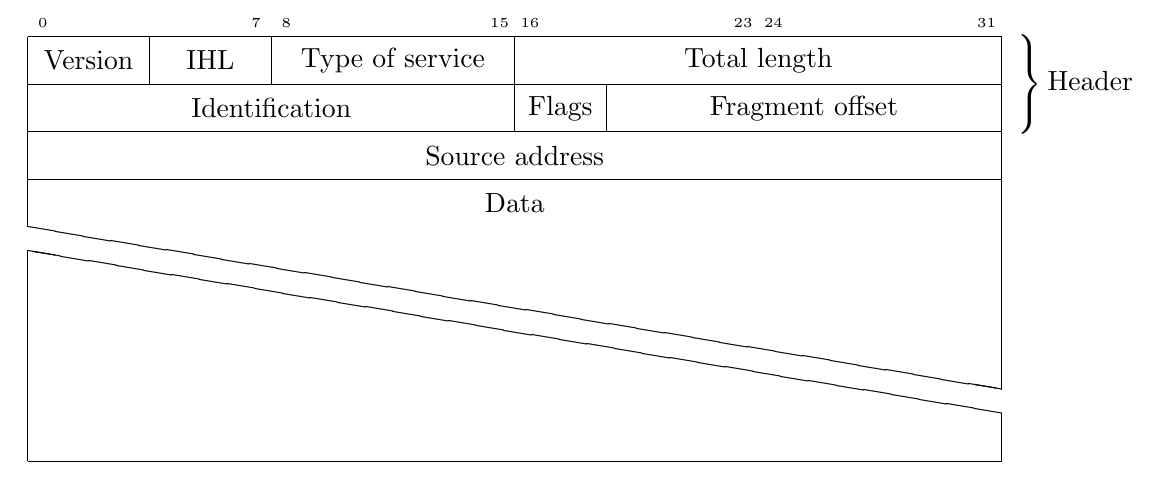
\begin{tikzpicture}[x=1cm, y=1cm]
  \node[inner sep=0pt] at (7.03,-2.91) {\pgfinterruptpicture%
  \begin{bytefield}[bitwidth=1.1em]{32}
    \bitheader{0,7,8,15,16,23,24,31} \\
    \begin{rightwordgroup}{Header}
      \bitbox{4}{Version} & \bitbox{4}{IHL} & \bitbox{8}{Type of service} & \bitbox{16}{Total length} \\
      \bitbox{16}{Identification} & \bitbox{3}{Flags} & \bitbox{13}{Fragment offset}
    \end{rightwordgroup} \\
    \wordbox{1}{Source address} \\
    \wordbox[lrt]{1}{Data} \\
    \skippedwords \\
    \wordbox[lrb]{1}{}
  \end{bytefield}%
  \endpgfinterruptpicture};
\end{tikzpicture}
\end{document}
